\documentclass[oneside]{memoir}
\let\STARTCODE\relax 
\let\STOPCODE\relax 
\STARTCODE
\usepackage{fourier} % or what ever
\usepackage[scaled=.92]{helvet}%. Sans serif - Helvetica
\usepackage{color,calc}
\usepackage{hyperref}
\usepackage{breakurl}
\usepackage{graphicx}
\usepackage{enumitem}
\usepackage{wrapfig}
\usepackage{listings}
\usepackage[fleqn]{amsmath}
\usepackage[usenames,dvipsnames]{xcolor}
\usepackage{fullpage}

\hypersetup{%
    pdfborder = {0 0 0}
}


\newsavebox{\ChpNumBox}
\definecolor{ChapBlue}{rgb}{0.00,0.65,0.65}
\makeatletter
\newcommand*{\thickhrulefill}{%
  \leavevmode\leaders\hrule height 1\p@ \hfill \kern \z@}
\newcommand*\BuildChpNum[2]{%
  \begin{tabular}[t]{@{}c@{}}
    \makebox[0pt][c]{#1\strut}  \\[.5ex]
    \colorbox{ChapBlue}{%
      \rule[-10em]{0pt}{0pt}%
      \rule{1ex}{0pt}\color{black}#2\strut
      \rule{1ex}{0pt}}%
  \end{tabular}}
\makechapterstyle{BlueBox}{%
  \renewcommand{\chapnamefont}{\large\scshape}
  \renewcommand{\chapnumfont}{\Huge\bfseries}
  \renewcommand{\chaptitlefont}{\raggedright\Huge\bfseries}
  \setlength{\beforechapskip}{20pt}
  \setlength{\midchapskip}{26pt}
  \setlength{\afterchapskip}{40pt}
  \renewcommand{\printchaptername}{}
  \renewcommand{\chapternamenum}{}
  \renewcommand{\printchapternum}{%
    \sbox{\ChpNumBox}{%
      \BuildChpNum{\chapnamefont\@chapapp}%
      {\chapnumfont\thechapter}}}
  \renewcommand{\printchapternonum}{%
    \sbox{\ChpNumBox}{%
      \BuildChpNum{\chapnamefont\vphantom{\@chapapp}}%
      {\chapnumfont\hphantom{\thechapter}}}}
  \renewcommand{\afterchapternum}{}
  \renewcommand{\printchaptertitle}[1]{%
    \usebox{\ChpNumBox}\hfill
    \parbox[t]{\hsize-\wd\ChpNumBox-1em}{%
      \vspace{\midchapskip}%
      \thickhrulefill\par
      \chaptitlefont ##1\par}}%
}
\chapterstyle{BlueBox}
\STOPCODE
\setlength\afterchapskip {\onelineskip }
\setlength\beforechapskip {\onelineskip }

\setlength{\parskip}{3pt}

\setcounter{secnumdepth}{2}

\setlist[itemize]{noitemsep, topsep=1pt}
\setlist[enumerate]{noitemsep, topsep=1pt}

\usepackage{listings}
\usepackage{color}

\definecolor{mygreen}{rgb}{0,0.6,0}
\definecolor{mygray}{rgb}{0.5,0.5,0.5}
\definecolor{mymauve}{rgb}{0.58,0,0.82}

\lstdefinestyle{Makefile}
{
    numberblanklines=false,
    language=make,
    tabsize=4,
    keywordstyle=\color{red},
    identifierstyle= %plain identifiers for make
}

\lstset{
    float=hbp,
    basicstyle=\ttfamily\footnotesize,
    keywordstyle= \color{blue} \textbf,
    stringstyle=\color{red},
    language=C++,
    tabsize=3,
    commentstyle=\color{BrickRed},
    columns=flexible,
    breaklines=true,
    extendedchars=\true,
    showstringspaces=false,
  numbers=left,
  numberstyle=\footnotesize,
  stepnumber=1,
  numbersep=5pt,
  frame=leftline,
  morekeywords={FlashSystem, ErrorManager, Param, Address, vector},
}

\setcounter{tocdepth}{2}

\counterwithout{section}{chapter}

\newcommand\numberthis{\addtocounter{equation}{1}\tag{\theequation}}

\begin{document}

\title{\textbf{Flash Layer Default Performance and Power Consumption Models}}
\author{Pierre Olivier <\href{mailto:pierre.olivier@univ-brest.fr}{pierre.olivier@univ-brest.fr}>}
\date{\today}

\maketitle

\tableofcontents

\chapter{Modeling Performance and Power Consumption of a NAND Flash Storage Subsystem}

\section{Introduction}

The equations presented here are used to model the performance (time taken) and energy consumed for the follwoing flash commands:

\begin{enumerate}
  \item Legacy read, write, erase ;
  \item Copy-back ;
  \item Cache read, cache write ;
  \item Multi plane read, write, erase ;
  \item Multi plane copy-back, multi plane cache read, multi plane cache write ;
  \item Lun-interleaved operations ;
  \item Multi channel operations.
\end{enumerate}

To do so, we use the variables and constants defined in Table \ref{table:constvars}.

\begin{table}[h!]
\center
\begin{tabular}{| c | p{6cm} | c | c |}
\hline
\textbf{name} & \textbf{description} & \textbf{unit} & \textbf{variable ?}\\
\hline
\hline
$TIN$ & Transfer In Nand, time taken to transfer of data (a page) from the page register to the NAND array in a plane. & $\mu$s & yes\\
\hline
$TON$ & Transfer Out of Nand, time taken to transfer of a page from the NAND array to the page register. & $\mu$s & yes\\
\hline
$IO$ & Time taken to transfer a page on the I/O bus. & $\mu$s & no\\
\hline
$BERS$ & Block ERaSe, time taken to erase a flash block. & $\mu$s & no\\
\hline
$PTIN$ & Power during $TIN$. & W & no\\
\hline
$PTON$ & Power during $TON$. & W & no\\
\hline
$PIO$ & Power during $IO$. & W & no\\
\hline
$PBERS$ & Power during block erase. & W & no\\
\hline
\end{tabular}
\caption{Variable and constants of our model}
\label{table:constvars}
\end{table}

We assume the following:

\begin{itemize}
  \item The time for sending commands opcodes and address is considered negligible, so it is not modeled ;
  \item Transfering a page from the page register on the I/O bus (read) takes the same time as transferring a page on the I/O bus to the page register (write). Time taken for these two operation is represented by $IO$ ;
  \item $TIN$ and $TON$ can be variable, according to the index of the addressed page in its block (in particular in MLC NAND). So in fact we have terms like $TIN_{addr}$ and $TON_{addr}$ representing the time taken to transfer a page to / from the nand array according to that page index within its containing block.
\end{itemize}

In this document, the unit of time is the microsecond. The unit of power is the watt, and the unit of energy is the microjoule.

\section{Models}

\subsection{Legacy Read}

An example of legacy read operation execution is presented on Figure \ref{fig:legrwe}.

\subsubsection{Performance}

\begin{align} T_{LegacyRead}(addr) = TON_{addr} + IO \end{align}

$addr$ is the address of the page being read, so $TON_{addr}$ represents the time to transfer this page from the NAND array to the page register.

\subsubsection{Energy Consumption}

\begin{align} E_{LegacyRead}(addr) = PTON*TON_{addr} + PIO*IO \end{align}

\subsection{Legacy Write}

An example of legacy write operation execution is presented on Figure \ref{fig:legrwe}.

\subsubsection{Performance}

\begin{align} T_{LegacyWrite}(addr) = IO + TIN_{addr} \end{align}

\subsubsection{Energy Consumption}

\begin{align} E_{LegacyWrite}(addr) = PIO*IO + PTIN*TIN_{addr} \end{align}

\subsection{Legacy Erase}

An example of legacy erase operation execution is presented on Figure \ref{fig:legrwe}.

\subsubsection{Performance}

\begin{align} T_{LegacyErase} = BERS \end{align}

\subsubsection{Energy Consumption}

\begin{align} E_{LegacyErase} = PBERS*BERS \end{align}

\begin{figure}
  \center
  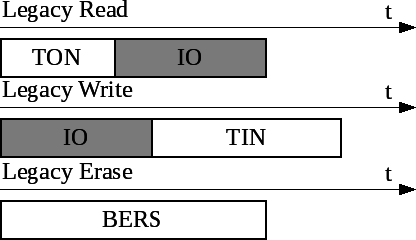
\includegraphics[width=0.6\textwidth]{Includes/LegacyReadWriteErase.png}
  \caption{Legacy read, write and erase operations execution}
  \label{fig:legrwe}
\end{figure}

\subsection{Copy-Back}

An example of copy back operation execution is presented on Figure \ref{fig:cbcrcw}.

\subsubsection{Performance}

\begin{align} T_{CopyBack}(src, dest) = TON_{src} + TIN_{dest} \end{align}

$src$ and $dest$ are the source (page read) and destination (page written) addresses of the copy-back operation.

\subsubsection{Energy Consumption}

\begin{align} E_{CopyBack}(src, dest) = PTON*TON_{src} + PTIN*TIN_{dest} \end{align}

\subsection{Cache Read}

An example of cache read operation execution is presented on Figure \ref{fig:cbcrcw}.

\subsubsection{Performance}

\begin{align}
T_{CacheRead}(addr_1, addr_2, ... , addr_n) = 
\notag\\TON_{page_1} + \sum\limits_{i=2}^{n} max(TON_{addr_i}, IO) + IO
\notag\\\text{with } n \ge 2
\end{align}

\subsubsection{Energy Consumption}

\begin{align} 
E_{CacheRead}(addr_1, addr_2, ... , addr_n) = \sum\limits_{i=1}^{n} (PTON*TON_{addr_i} + PIO*TIO)
\notag\\\text{with } n \ge 2
\end{align}

$addr_1, ... , addr_n$ are the addresses of the different pages being read sequentially during the cache read operation. Note that $n$ must be at least 2.

\subsection{Cache Write}

An example of cache write operation execution is presented on Figure \ref{fig:cbcrcw}.

\subsubsection{Performance}

\begin{align} 
T_{CacheWrite}(addr_1, addr_2, ... , addr_n) = 
\notag\\IO + \sum\limits_{i=2}^{n} max(TIN_{addr_i}, IO) + TIN_{addr_n}
\notag\\\text{with } n \ge 2
\end{align}

\subsubsection{Energy Consumption}

\begin{align} E_{CacheWrite}(addr_1, addr_2, ... , addr_n) = 
\notag\\\sum\limits_{i=1}^{n} (PTIN*TIN_{addr_i} + PIO*TIO) 
\notag\\\text{with } n \ge 2
\end{align}

\begin{figure}
  \center
  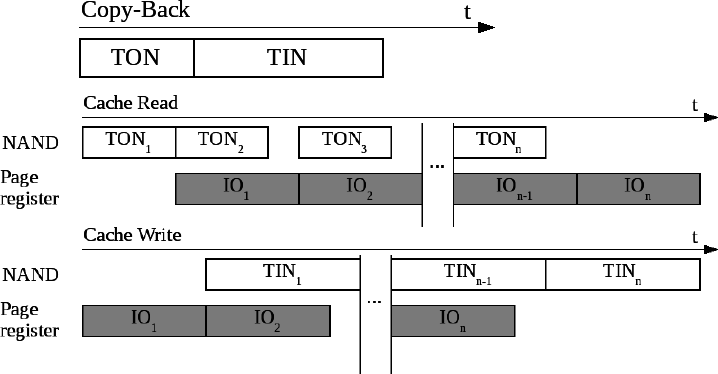
\includegraphics[width=0.7\textwidth]{Includes/CopyBackCacheReadWrite.png}
  \caption{Copy-back, cache read and cache write operations execution}
  \label{fig:cbcrcw}
\end{figure}

\subsection{Multi Plane Read}

An example of multi plane read operation execution is presented on Figure \ref{fig:mprmpwmpe}.

\subsubsection{Performance}

  We define $T_{P_i}$ as the time of one read operation in the plane $i$:
\begin{align} 
T_{P_1}(addr_1) &= TON_{addr_1} + IO
\notag\\T_{P_i}(addr_i) &= max(T_{P_{i-1}}, TON_{addr_i}) + IO
\end{align}

$addr_i$ is the address of the page to read in the plane $i$. So we have:
\begin{align} T_{MultiPlaneRead}(addr_1, addr_2, ... , addr_n) = max_i(T_{P_i})
\notag\\\text{with } n \ge 2
\end{align}
  
$n$ is the number of planes participating in the multi plane operation.
  
\subsubsection{Energy Consumption}
\begin{align} E_{MultiPlaneRead}(addr_1, addr_2, ... , addr_n) = 
\notag\\\sum\limits_{i=1}^{n}(PTON*TON_{addr_i}) + n*PIO*IO 
\notag\\&\text{with } n \ge 2
\end{align}

\subsection{Multi Plane Write}

An example of multi plane write operation execution is presented on Figure \ref{fig:mprmpwmpe}.

\subsubsection{Performance}

  $T_{P_i}$ is the time of one write operation in the plane $i$. It is defined as follows:
\begin{align} T_{P_i} (addr_i) = i*IO + TIN_{addr_i} \end{align}

  $addr_i$ is the address of the page to write in plane $i$. So we have:
  
\begin{align} T_{MultiPlaneWrite}(addr_1, addr_2, ... , addr_n) &= max_i(T_{P_i})
\notag\\ &= max_i(i*IO + TIN_{addr_i})
\notag\\&\text{with } n \ge 2
\end{align}

$n$ is the number of planes participating in the multi plane operation.
  
  \subsubsection{Energy consumption}

\begin{align} 
E_{MultiPlaneWrite}(addr_1, addr_2, ... , addr_n) = 
\notag\\n*PIO*IO + \sum\limits_{i=1}^{n} (PTIN*TIN_{addr_i})
\notag\\&\text{with } n \ge 2
\end{align}

\subsection{Multi Plane Erase}

An example of multi plane erase operation execution is presented on Figure \ref{fig:mprmpwmpe}.

\subsubsection{Performance}

\begin{align} 
T_{MultiPlaneErase}(addr_1, addr_2, ... , addr_n) = BERS
\notag\\\text{with } n \ge 2
\end{align}

$n$ is the number of planes participating in the multi plane operation.

\subsubsection{Energy Consumption}

\begin{align}
E_{MultiPlaneErase}(addr_1, addr_2, ... , addr_n) = n*PBERS*BERS
\notag\\\text{with } n \ge 2
\end{align}

\begin{figure}
  \center
  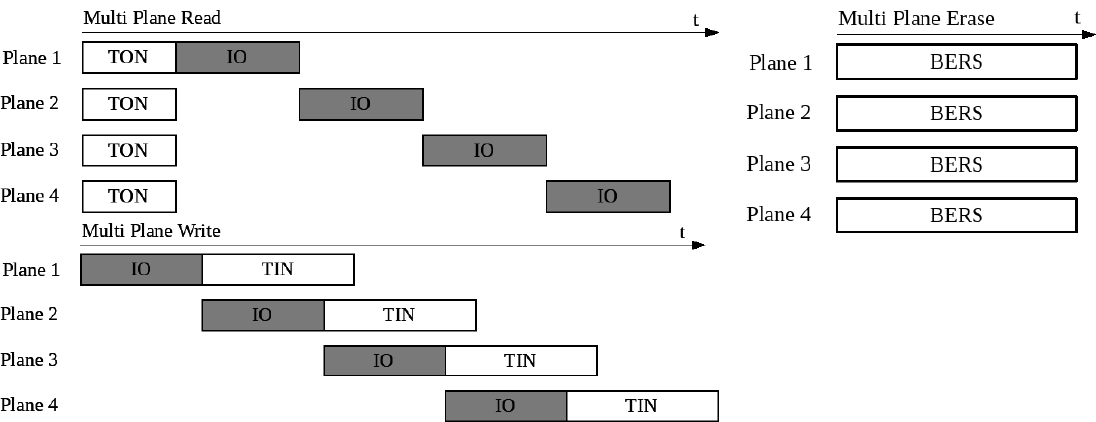
\includegraphics[width=0.9\textwidth]{Includes/MultiPlaneReadWriteErase.png}
  \caption{Multi plane read, write and erase operations execution}
  \label{fig:mprmpwmpe}
\end{figure}

\subsection{Multi Plane Copy-Back}

\subsubsection{Performance}

\begin{align}
T_{MultiPlaneCopyBack}(src_1, src_2, ... , src_n, dest_1, dest_2, ... , dest_n) = 
\notag\\max_i (TON_{src_i} + TIN_{dest_i})
\notag\\\text{with } n \ge 2
\end{align}

$n$ is the number of planes participating in the multi plane operation.

\subsubsection{Energy Consumption}

\begin{align}
E_{MultiPlaneCopyBack}(src_1, src_2, ... , src_n, dest_1, dest_2, ... , dest_n) = 
\notag\\\sum\limits_{i=1}^{n} (PTON*TON_{src_i} + PTIN*TIN_{dest_i})
\notag\\\text{with } n \ge 2
\end{align}

\subsection{Multi Plane Cache Read and Multi Plane Cache Write}

The multi plane cache read and write operations can be caracterized as a set of lists of addresses. Each list represent a cache read / write operation in one plane. So the is one list per plane participating in the multi plane cache operation. Each list contains the addresses of the pages to read or write sequentially for the corresponding cache operation. For example, a multi plane cache operation on four plane with three pages read / written sequentially in each plane can be described as follows:
\begin{align} [ addr_{1,1}, addr_{1,2}, addr_{1,3}, addr_{2,1}, addr_{2,2}, addr_{2,3}, addr_{3,1}, 
\notag\\addr_{3,2}, addr_{3,3}, addr_{4,1}, addr_{4,2}, addr_{4,3} ] \end{align}

$addr_{i,j}$ represents the address of the $j$-th page to read / write in plane $i$. The multi plane cache read operation has one $TON_{i,j}$ and one $IO_{i,j}$ related to each page read. Similarly, the multi plane cache write operation has one $IO_{i,j}$ and one $TIN_{i,j}$ for each page written. Those values are depicted on the example of multi plane cache read and write on Figure \ref{fig:mpcr} and Figure \ref{fig:mpcw}. Note that $IO$ is a constant, therefore each $IO_{i,j}$ is actually equal to $IO$ (with the exeception when $addr_{i,j}$ is $none$, as explained below). However, $TON_{i,j}$ and $TIN{i,j}$ are variables.

\begin{figure}
  \center
  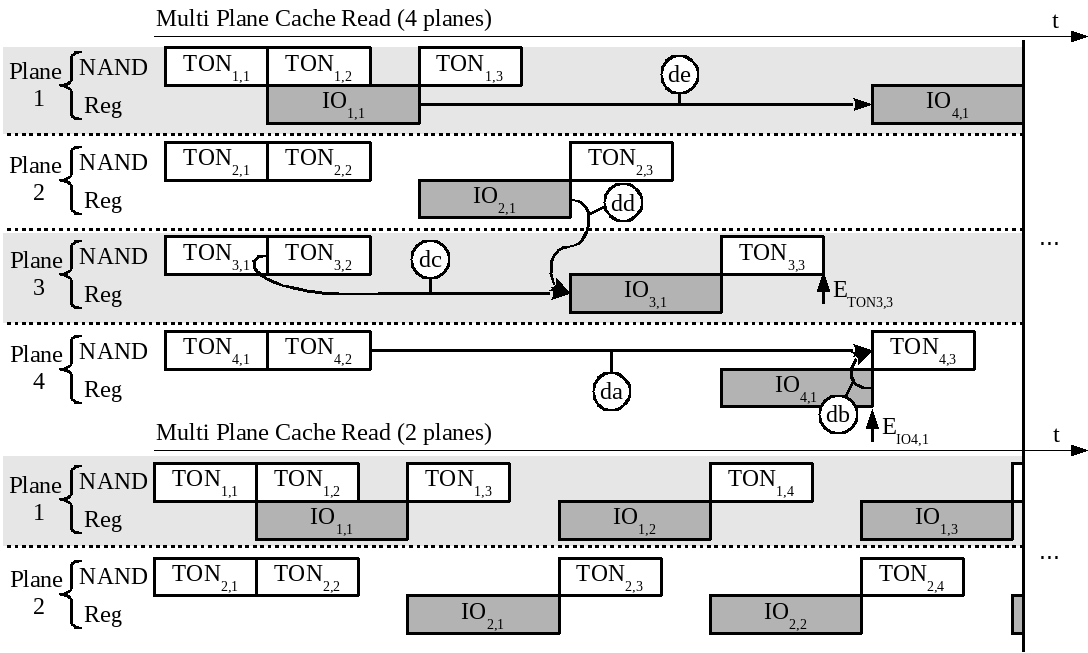
\includegraphics[width=0.9\textwidth]{Includes/MultiPlaneCacheRead.png}
  \caption{Multi plane cache read operation execution}
  \label{fig:mpcr}
\end{figure}

\begin{figure}
  \center
  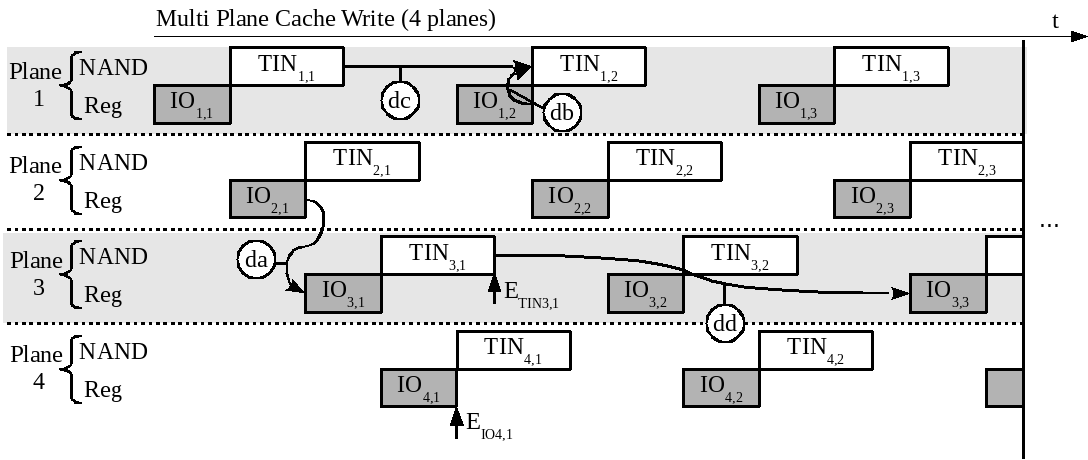
\includegraphics[width=0.9\textwidth]{Includes/MultiPlaneCacheWrite.png}
  \caption{Multi plane cache write operation execution}
  \label{fig:mpcw}
\end{figure}

In the case which the number of page to read / write sequentially is different from one plane to another, the size of each list is set to the size of the biggest list. We introduce the term $none$, used to fill the 'holes' in smaller lists. For example, a multi plane cache operation on two planes, with four pages accessed sequentially in the first plane, and only two pages accessed sequentially in the second, will be represented as follows:
\begin{align} [ addr_{1,1}, addr_{1,2}, addr_{1,3}, addr_{1,4}, addr_{2,1}, addr_{2,2}, addr_{2,3}=none, \notag\\addr_{2,4}=none ] \label{eq:none}\end{align}

$none$ terms will be useful in the performance / power consumption computation: we define that $TON$, $IO$ and $TIN$ values for an address equal to $none$ as $0$:
\begin{align}
TON_{i,j} & =
\begin{cases}
      TON_{addr_{i,j}} & \text{if } addr_{i,j} \ne none\\
      0 & \text{otherwise}
\end{cases}\\
TIN_{i,j} & =
\begin{cases}
      TIN_{addr_{i,j}} & \text{if } addr_{i,j} \ne none\\
      0 & \text{otherwise}
\end{cases}\\
IO_{i,j} & = 
\begin{cases}
      IO & \text{if } addr_{i,j} \ne none\\
      0 & \text{otherwise}
\end{cases}
\end{align}

We also define, for multi plane cache read / write operations, the terms $E_{TON_{i,j}}$, $E_{IO_{i,j}}$ and $E_{TIN_{i,j}}$. They are respectively the moments in time were the $TON$, $IO$ and $TIN$ operation just finished for the related page read / write. $E_{TON_{3,3}}$ and $E_{IO_{4,1}}$ are illustrated as an example on Figure \ref{fig:mpcr}. $E_{TIN_{3,1}}$ is illustrated on Figure \ref{fig:mpcw}.

In the following equations, $n$ is the number of planes participating in the multi plane cache read / write operation, and $m_i$ is the number of pages read / written in plane $i$. $m_max$ is the number of page read / written in plane containing the most important set of pages accessed. For our example presented in the expression \ref{eq:none}, $n=2$, $m_1=4$, $m_2=2$, and $m_{max}=max_i(m_i)=m_1=4$.

\subsubsection{Multi Plane Cache Read - Performance}

\noindent $E_{TON_{i,j}}$ depends of:

\begin{enumerate}
  \item $E_{IO_{i,j-2}}$ (db on Figure \ref{fig:mpcr}): the cache register containing page $(i,j-2)$ must be first emptied. It is then filled with page $(i,j-1)$, coming from the page register. As the page register is emptied, $TON_{i,j}$ can occur ;
  \item $E_{TON_{i,j-1}}$ (da on Figure \ref{fig:mpcr}) ;
  \item $TON_{i,j}$.
\end{enumerate}

\noindent $E_{IO_{i,j}}$ depends of:

\begin{enumerate}
  \item $E_{IO_{i-1,j}}$ (dd on Figure \ref{fig:mpcr}): the IO bus must be free ;
  \item $E_{TON_{i,j}}$ (dc on Figure \ref{fig:mpcr}): the page to output must be in the cache register ;
  \item $E_{IO_{i,j-1}}$ (de on Figure \ref{fig:mpcr}) ;
  \item $IO_{i,j}$.
\end{enumerate}

According to this, the execution time of the multi plane cache read operation can be modelled as follows:
\begin{align} 
E_{IO_{1,1}} &= TON_{1,1} + IO
\notag\\E_{IO_{1,j}} &= max(E_{IO_{n,j-1}}, E_{TON_{1,j}}, E_{IO_{i,j-1}}) + IO &\text{ with }j \ne 1
\notag\\E_{IO_{i,j}} &= max(E_{IO_{i-1,j}}, E_{TON_{i,j}}, E_{IO_{i,j-1}}) + IO &\text{ with }j \ne 1\text{ and }i \ne 1
\\\notag\\E_{TON_{i,1}} &= TON_{i,1}
\notag\\E_{TON_{i,2}} &= E_{TON_{i,1}} + TON_{i,2}
\notag\\E_{TON_{i,j}} &= max(E_{IO_{i,j-2}}, E_{TON_{i,j-1}}) + TON_{i,j} &\text{ with }j > 2 
\end{align}

\text{Finally: }
\begin{align}
T_{MultiPlaneCacheRead} (addr_{1,1}, addr_{1,2}, ... , addr_{1,m_{max}},
\notag\\ addr_{2,1}, ... , addr_{n,m_{max}}) = max_i(E_{IO_{i,m_{max}}})
\notag\\\text{with } n \ge 2 \text{ and } m_{max} \ge 2
\end{align}

\subsubsection{Multi Plane Cache Read - Energy Consumption}

\begin{align}
E_{MultiPlaneCacheRead} (addr_{1,1}, addr_{1,2}, ... , addr_{1,m_{max}}, 
\notag\\addr_{2,1}, ... , addr_{n,m_{max}}) = \sum\limits_{i=1}^{n} [\sum\limits_{j=1}^{m_{max}} (TON_{addr_{i,j}}*PTON + IO_{i,j}*PIO)]
\notag\\\text{with } n \ge 2 \text{ and } m_{max} \ge 2
\end{align}

\subsubsection{Multi Plane Cache Write - Performance}

$E_{TIN_{i,j}}$ depends of:
\begin{enumerate}
  \item $E_{TIN_{i,j-1}}$ (dc on Figure \ref{fig:mpcw}) ;
  \item $E_{IO_{i,j}}$ (db on Figure \ref{fig:mpcw}): IO transfer from the host must be complete to then load the page in the NAND array ; 
  \item $TIN_{i,j}$.
\end{enumerate}

$E_{IO_{i,j}}$ depends of:
\begin{enumerate}
  \item $E_{IO_{i-1,j}}$ (da on Figure \ref{fig:mpcw}): the IO bus must be free for the IO transfer of page $(i, j)$ ;
  \item $E_{TIN_{i,j-2}}$ (dd on Figure \ref{fig:mpcw}): when the page ($i,j-2$) is fully transfered to the NAND array, the page register is empty. So the page ($i, j-1$) can be placed in that page register, coming from the cache register. Then, as the cache register is empty, $TIN_{i,j}$ can occur. ;
  \item $IO_{i,j}$.
\end{enumerate}

The execution time of the multi plane cache write operation can the be modelled as follows:

\begin{align}
E_{IO_{1,1}} &= IO_{i,j}
\notag\\E_{IO_{1,j}} &= E_{IO_{n,j-1}} + IO_{i,j} &\text{with } 2 \le j \le 3
\notag\\E_{IO_{1,j}} &= max(E_{IO_{n,j-1}}, E_{TIN_{1, j-2}}) + IO_{i,j} &\text{with } j > 3
\notag\\E_{IO_{i,j}} &= E_{IO_{i-1,j}} + IO_{i,j} &\text{with } i \ne 1 \text{ and } 2 \le j \le 3
\notag\\E_{IO_{i,j}} &= max(E_{IO_{i-1,j}}, E_{TIN_{i, j-2}}) + IO_{i,j} &\text{with } i \ne 1 \text{ and } j > 3
\\
\notag\\E_{TIN_{1,1}} &= E_{IO_{1,1}} + TIN_{1,1}
\notag\\E_{TIN_{i,j}} &= max(E_{IO_{i,j}}, E_{TIN_{i,j-1}}) + TIN_{i,j} &\text{with } i \ne 1 \text{ and } j \ne 1
\end{align}

Once again here $n$ is the number of planes participating in the multi plane operation. Finally we have:
\begin{align}
T_{MultiPlaneCacheWrite} (addr_{1,1}, addr_{1,2}, ... , addr_{1,m_{max}}, 
\notag\\addr_{2,1}, ... , addr_{n,m_{max}}) = max_i(E_{TIN_{i, m_{max}}})
\notag\\\text{with } n \ge 2 \text{ and } m_{max} \ge 2
\end{align}


\subsubsection{Multi Plane Cache Write - Energy Consumption}
\begin{align}
E_{MultiPlaneCacheWrite} (addr_{1,1}, addr_{1,2}, ... , addr_{1,m_{max}}, 
\notag\\addr_{2,1}, ... , addr_{n,m_{max}}) = 
\sum\limits_{i=1}^{n} [\sum\limits_{j=1}^{m_{max}} (TIN_{addr_{i,j}}*PTIN + IO_{addr_{i,j}}*PIO)]
\notag\\\text{with } n \le 2 \text{ and } m_{max} \le 2
\end{align}

\subsection{LUN-interleaved commands}

\subsubsection{Performance}

\subsubsection{Energy Consumption}

\subsection{Multi Channel}

\subsubsection{Performance}

\begin{align}T_{MultiChannel}(cmd_1, cmd_2, ... , cmd_n) = max_i(T_{cmd_i})
\notag\\\text{with } n \ge 2
\end{align}

$n$ is the number of channels participating in the multi channel operation.\\$cmd_1, ... , cmd_n$ are the commands sent in parallel amongst different channels. $T_{cmd_i}$ is the time required to process $cmd_i$, computed using one of the previously presented equations.

\subsubsection{Energy Consumption}

\begin{align} E_{MultiChannel}(cmd_1, cmd_2, ... , cmd_n) = \sum\limits_{i=1}^n E_{cmd_i}
\notag\\\text{with } n \ge 2
\end{align}

$E_{cmd_i}$ represents the energy consumed during the execution of $cmd_i$, computed using the previously presented equations.

\end{document}

